\chapter{Electric Potential}

Shuffle across a carpet in socks and touch a doorknob, and a spark jumps. A thunderstorm does the same thing
on a scale of a billion volts. In the Charge chapter, you learned how charges push and pull
on each other through electric fields. This chapter looks at the same forces through the lens of energy: how
much energy a charge gains or loses as it moves through a field, and what a ``volt'' really measures.

\section{Electric Potential}
A ball held above the ground has gravitational potential energy; let it
go, and gravity turns that into kinetic energy. Charges work the same way.
A charge in an electric field has \textbf{electric potential
energy}\index{electric potential energy} $U_E$. When the field does work
$W_E$ on the charge, its potential energy drops by the same amount:
\begin{equation}
	\Delta U_E = -W_E \label{eq:change_in_epe}
\end{equation}

Notice how this is similar to an object of mass $m$ undergoing work done by a gravitational field $\Delta U_G = -W_G$.

\begin{Exercise}[title={Change in Electric Potential Energy}, label={eq:electric_potential_energy}]

A positive charge $+q$ moves a distance $r$ from position $X$ to position $Y$ in a \textbf{uniform} electric field $E$.


\begin{tikzpicture}[scale=2]

  \foreach \y in {-0.5, 0.0, 0.5} {
    \draw[->, >=Stealth, thick, densely dashed, gray] (0,\y) -- (3,\y);
  }
 
  \coordinate (X) at (0.25,0); % Point X is at x=1
  \coordinate (Y) at (2.25,0); % Point Y is at x=2

  \node[above=2pt of X] {\textbf{X}};
  \node[above=2pt of Y] {\textbf{Y}};

  \draw[->, >=Triangle, thick] (X) -- node[midway, below=3pt] {\textit{r}} (Y);

  \node[right=2pt] at (3,0) {\textbf{E}};

\end{tikzpicture}

What is its change in electric potential energy? Assume moving in direction $r$ moves in the direction of $E$.
\end{Exercise}

\begin{Answer}[ref={eq:electric_potential_energy}]

Since the field is uniform, the charge has a constant electric force felt on it: $\vec{\mathbf{F}}_E=q \vec{\mathbf{E}}$. Since $q$ is positive, $\vec{\mathbf{F}}_E$ points in the same direction as $\vec{\mathbf{E}}$. Because the force and the displacement $r$ are in the same direction, the work $W_E$ done by the electric field is positive:

$$W_E = F_E \cdot r = qEr$$

Thus the change in electric potential energy is
$$\Delta U_E = -qEr$$
It is \emph{negative} because when the field does positive work, the
potential energy goes down.
\end{Answer}

\index{electric potential}\textbf{Electric potential} $V$ is the
electric potential energy per unit charge: $V = \frac{U_E}{q}$. It is
measured in volts (1 volt = 1 joule per coulomb). Potential belongs to a
\emph{place}, whether or not a charge is there, the same way height
belongs to a spot on a hill whether or not a ball is sitting there.

Just as moving a mass up in height against gravity increases its gravitational potential, moving a positive charge "up" against an electric field increases its electric potential. In both cases, the field \textit{tries} to push the object toward a state of lower potential energy. A positive charge naturally wants to move with the electric field toward lower potential; in this case, its electric potential energy is converted into kinetic energy. Conversely, to move a positive charge against an electric field, work must be done on the charge, causing its electric potential to increase.

Moving from two points not on the same electric field line introduces an angle component $\theta$:

\begin{wrapfigure}{l}{4in}
	\begin{tikzpicture}[scale=2]
		% Electric Field lines (E)
		\foreach \y in {-0.5, 0.0, 0.5} {
			\draw[->, thick, densely dashed, gray] (0,\y) -- (3,\y);
			}
			\node[right=5pt] at (3,0) {\textbf{E}};
			
			% Points a and b
			\coordinate (a) at (0.25,-0.5); 
			\coordinate (b) at (2.25,0.5); 
			\coordinate (a_ext) at (1.25, -0.5); % Helper point for angle
			
			\node[below left=2pt of a] {\textbf{a}};
			\node[above right=2pt of b] {\textbf{b}};
			\fill (a) circle (0.5pt);
			\fill (b) circle (0.5pt);
			
			\draw[->, thick] (a) -- node[midway, above left] {\textit{r}} (b);
			
			\pic [draw, "$\theta$", angle eccentricity=1.5, angle radius=0.6cm] {angle = a_ext--a--b};
			
			\draw[|<->|, thick] (0.25, -1.0) -- node[below=2pt] {$r \cos \theta$} (2.25, -1.0);
			\draw[dotted, gray] (a) -- (0.25, -1.0);
			\draw[dotted, gray] (b) -- (2.25, -1.0);
			
		\end{tikzpicture}
		\caption{A gain of potential energy across an angle.}
		\label{fig:elec_pe_1}
	\end{wrapfigure}

% knowledge of line integrals does not exist 
The \index{potential difference}electric potential difference between two points $A$ and $B$ is defined by the line integral of the electric field:
\begin{equation}
    \Delta V = V_B - V_A = -\int_{A}^{B} \vec{\mathbf{E}} \cdot d\vec{\mathbf{l}}
\end{equation}
The negative sign indicates that the potential decreases in the direction of the electric field.

We can easily define two point charges $q_1$ and $q_2$ separated by distance $r$ to have potential energy
\begin{equation}
	U=k\frac{q_1q_2}{r}=\frac{1}{4\pi \epsilon_0}\frac{q_1q_2}{r}
\end{equation}
\begin{Exercise}[title={Accelerating an Electron}, label={ex:electron_accel_epd}]
	\textit{This is a sample problem from an IB Physics Exam}.
	% https://github.com/user-attachments/files/24828324/Physics_paper_2_TZ1_HL.pdf
An electron is accelerated from rest by an electric potential difference $V$. The electron reaches a speed of $9.4 \times 10^6 \, \textrm{m/s}$. Using the charge of an electron as $e = 1.6 \times 10^{-19} \, \textrm{C}$ and the mass of an electron as $m_e = 9.11 \times 10^{-31} \, \textrm{kg}$, find the potential difference $V$ that accelerated the electron to this speed. You may use a calculator to simplify computations.
\end{Exercise}
\begin{Answer}[ref={ex:electron_accel_epd}]

Using our equations, we can derive an equation for the potential difference $V$:
\begin{align*}
	\Delta U_E &= q\Delta V \\
	W_E &= \Delta U_E \\
	W_E &= qV \\
	\text{gain in kinetic energy} &= \text{work done by field} \\
	\frac{1}{2}mv^2 &= qV \\
	V &= \frac{1}{2}\frac{mv^2}{q}
\end{align*}

Since our we are given the speed, and the charge and mass of the electron, we can plug in our values:
\begin{align*}
	V&=\frac{\frac12(9.11\times10^{-31})(9.4\times10^6)^2}{1.60\times10^{-19}}\\
	&=\frac{\frac12(9.11\times10^{-31})(8.836\times10^{13})}{1.60\times10^{-19}}\\
	&=\frac{\frac12 (8.05\times10^{-17})}{1.60\times10^{-19}}\\
	&=\frac{4.03\times10^{-17}}{1.60\times10^{-19}}\\
	&=252 \, \textrm{V}
\end{align*}
A potential difference of about 252 volts does the job. (Since an electron
is negative, it speeds up when it moves toward \emph{higher} potential.)
\end{Answer}
\subsection{Point Charges, Uniform Fields, and Spherical Shells}
In a \textbf{uniform electric field} (such as the space between two large parallel plates), the field strength $E$ is constant. The potential difference between two points separated by a distance $d$ along the field lines is:
\begin{equation}
    \Delta V = -Ed
\end{equation}
For a \textbf{point charge} $Q$, we typically set the reference point ($V=0$) at infinity. The potential at a distance $r$ from the charge is:
\begin{equation}
    V = \frac{1}{4\pi\epsilon_0} \frac{Q}{r}
	\label{eq:point_charge}
\end{equation}
Unlike the electric field, which is a vector and follows an $1/r^2$ factor, electric potential is a \textbf{scalar} and follows an $1/r$ factor.
\subsection*{Surface Spherical Charge}
For all spherical objects of radius $R$ (surface spheres - assume hollow interior), it has potential inside and outside of the shell. For all points outside the shell, it is the same for any point charge $Q$, as seen in equation~\ref{eq:point_charge}. For all points \emph{inside} the shell, the potential is
$$V = \frac{1}{4\pi\epsilon_0} \frac{Q}{R}$$
This means that moving a test charge $q$ from the surface of the shell to the center of the shell, the potential does not change. The potential is constant within the shell.

If the charge is spread evenly through a \emph{solid} sphere instead, the
potential inside at distance $r$ from the center is
$$V = \frac{1}{4\pi\epsilon_0}\frac{Q}{2R} \left(3 - \frac{r^2}{R^2}\right)$$

\subsection{Potential due to Configurations of Charge}
Because potential is a scalar, finding the total potential from multiple charges is often simpler than finding the total electric field. We do not need to worry about components, instead, we simply sum the potentials:
\begin{equation}
    V = \sum_i \frac{k q_i}{r_i} \quad \text{or for continuous distributions} \quad V = k \int \frac{dq}{r}
\end{equation}

\subsection{Conservation of Energy}
When a charge $q$ moves through a potential difference $\Delta V$, the change in its electric potential energy is $\Delta U_E = q\Delta V$. If no other forces are acting on the charge, the total mechanical energy is conserved:
\begin{equation}
    K_a + U_{E,a} = K_b + U_{E,b} \implies \frac{1}{2}mv_a^2 + qV_a = \frac{1}{2}mv_b^2 + qV_b
\end{equation}
\subsection{Summary}
\begin{table}[H]
    \centering
    \begin{tabular}{|l|l|l|l|}
    \hline
        Particle & \textit{wants} to move toward\dots & Potential Change ($\Delta V$) & Potential Energy Change ($U_E$​) \\ \hline
        Positive ($+q$) & Lower Potential & Negative (Decreases) & Negative (Decreases) \\ \hline
        Negative ($-q$) & Higher Potential & Positive (Increases) & Negative (Decreases) \\ \hline
    \end{tabular}
\end{table}

\begin{Exercise}[title={Electron between Field Plates}, label={ex:electron_field_plates}]
	\textit{This is a sample problem from an IB Physics Exam}.
	An electron that is travelling at a horizontal speed $v_x = 9.4\times10^6 \textrm{ms}^{-1}$ now enters a region of a \textit{uniform electric field} between two parallel charged plates, separated by a distance of $4.0 \, \textrm{cm}$. The electron is initially halfway between the plates and its initial velocity is parallel to the plates. The upper plate is positively charged and the lower plate is negatively charged. There is a potential difference between the plates of $V = 30 \, \textrm{V}$.

	Find the horizontal distance travelled before hitting a plate. Which plate does the electron hit?

\end{Exercise}
\begin{Answer}[ref={ex:electron_field_plates}]
First off, why do we know that the electron will hit a plate? Because the electric field between the plate exerts a force on the electron. The electron is attracted to the \textbf{positively} charged upper plate, so it will accelerate upwards and eventually hit the upper plate. Let us first find the acceleration caused by the electric field. The electric field strength $E$ between two parallel plates is given by:	
\begin{equation}
	E = \frac{V}{d} = \frac{30}{0.040} = 750 \, \textrm{V m}^{-1}
\end{equation}
Converting this to solve for the electron's acceleration:
\begin{equation}
	a = \frac{F}{m} = \frac{qE}{m} = \frac{(1.6\times10^{-19})(750)}{9.11\times10^{-31}} \approx 1.32\times10^{14} \, \textrm{m s}^{-2}
\end{equation}


To find the horizontal distance travelled, we use the vertical motion to find time, and then use that time to find the horizontal distance travelled. The vertical motion is a simple kinematics problem with constant acceleration:
\begin{align*}
	y &= v_{y0}t + \frac{1}{2}a_yt^2 \\
	0.02 &= 0 + \frac{1}{2}(1.32\times10^{14})t^2 \\
	t^2 &= \frac{0.04}{1.32\times10^{14}} \\
	t &\approx 1.74\times10^{-8} \, \textrm{s}	
\end{align*}	
Then, putting this into a horizontal motion equation:
\begin{align*}
	x &= v_{x0}t \\
	&= (9.4\times10^6)(1.74\times10^{-8}) \\
	&\approx 0.16 \, \textrm{m}
\end{align*}
So the electron travels a horizontal distance of about \textbf{0.16 meters} before hitting the upper plate.
\end{Answer}
\section{Lightning}\index{lightning}
A thundercloud is a tower of water droplets, ice crystals, and soft hail
(called graupel), churned by powerful updrafts. When small ice crystals
collide with heavier graupel, electrons are rubbed off, just like the
balloon on your hair. The heavy, negatively charged graupel sinks toward
the bottom of the cloud, while the light, positively charged ice crystals
are carried to the top.

Air is a good insulator, so at first the charge has nowhere to go. But it
keeps building until the electric field is strong enough to rip electrons
off air molecules, turning a path of air into a conductor. Then the charge
rushes through in a giant spark: lightning. It often strikes the tallest
object around, because that is the shortest path.
A great deal of lightning moves within a cloud or between clouds. However, sometimes
it jumps to the earth. These bolts of lightning vary in the amount of electrons
they carry, but the average is about 15 coulombs.
% ADD: Add water density explanation. ice less dense than liquid water due to crystalline structure.
\begin{figure}[H]
	\centering
	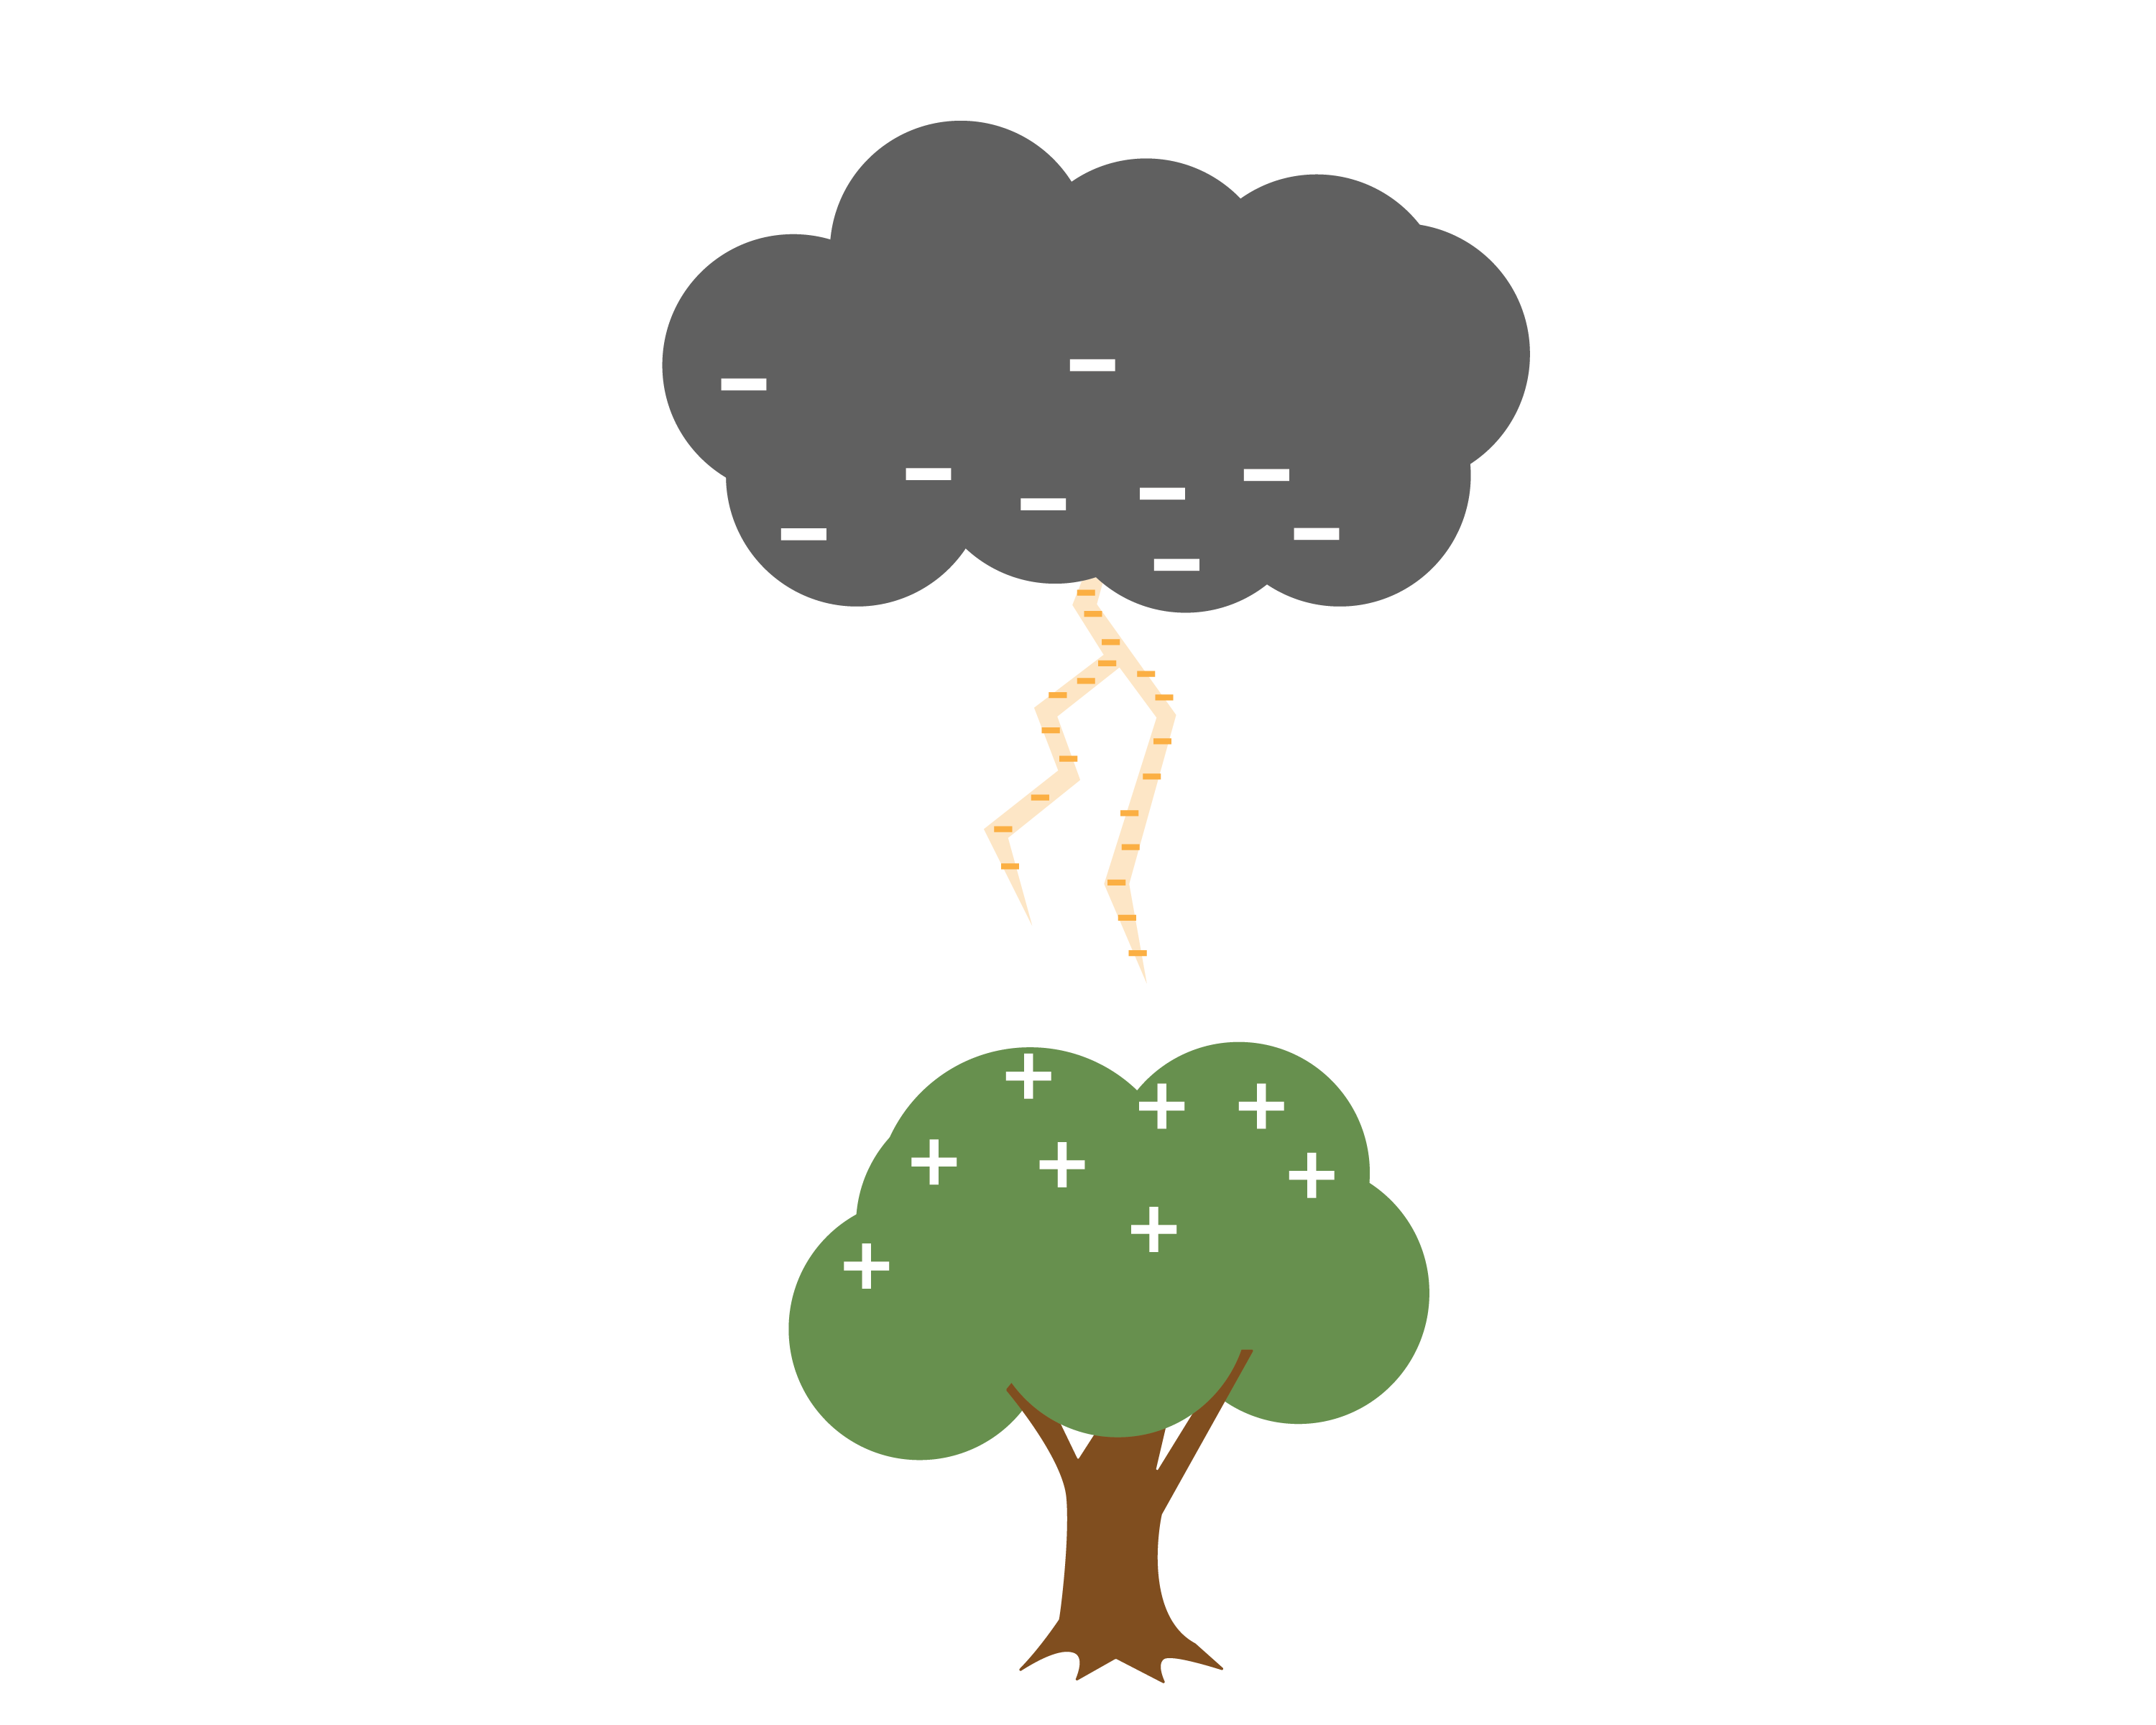
\includegraphics[width=1\textwidth]{lightning.png}
	\caption{A difference of charge causes a spark of lightning to generate and transfer.}
	\label{fig:lightning_img}
\end{figure}


Thunder occurs because the lightning heats the air it passes through to
about 30,000 kelvins, five times hotter than the surface of the Sun, so
the air expands explosively. The resulting shockwave is the sound we know as thunder.
% ADD: Relate speed of light and sound
